\documentclass[sigconf]{acmart}

\usepackage{xspace}
\usepackage{graphics}
\usepackage[T1]{fontenc}
\usepackage{times}
\usepackage{color}
\usepackage{booktabs}
\usepackage{textcomp}
\usepackage{microtype}
\usepackage{hyperref}
\usepackage{url}
\usepackage{relsize}
\usepackage{caption}
\usepackage{array}
\usepackage{ragged2e}
\usepackage{tabularx}
\usepackage{tikz}
\usetikzlibrary{positioning,arrows.meta,calc}

\hypersetup{
  colorlinks,
  urlcolor=blue}
\renewcommand*{\UrlFont}{\ttfamily\smaller\relax}

\AtBeginDocument{%
  \providecommand\BibTeX{{%
    \normalfont B\kern-0.5em{\scshape i\kern-0.25em b}\kern-0.8em\TeX}}}

\setcopyright{none}
\renewcommand\footnotetextcopyrightpermission[1]{}
\settopmatter{printacmref=false}

\newcolumntype{Y}{>{\RaggedRight\arraybackslash}X}
\newcommand{\tbl}{%
  \scriptsize
  \setlength{\tabcolsep}{4pt}%
  \renewcommand{\arraystretch}{1.12}%
}

\begin{document}
\pagestyle{plain}

\title{From Data Discovery to Analytics-Ready Data:\\A Survey of Search, Preparation, and Integration in Data Lakes}

\author{Sumaiya Azad}
\affiliation{%
  \institution{University of Utah}
  \city{Salt Lake City}
  \state{Utah}
  \country{USA}}
\email{sumaiya.azad@utah.edu}

\renewcommand{\shortauthors}{Azad}

\begin{abstract}
Data lakes promise flexible storage, but analysts rarely receive data in a form ready for dashboards, statistical analysis, or machine learning. Between raw lake contents and analytics-ready outputs, users must discover relevant sources, prepare noisy and heterogeneous data, and integrate partially overlapping tables. This literature review organizes recent work into three phases: Discovery and Search, Preparation and Wrangling, and Integration and Matching. It summarizes representative methods, explains the basis of the taxonomy, compares trade-offs in accuracy, automation, scalability, and human effort, and highlights open problems in end-to-end evaluation, safe automation, governance, and evolving data. The review shows how current systems move from data-lake search to usable analytical datasets, and where important research gaps remain.
\end{abstract}

\maketitle

\section{Introduction}
Data lakes store heterogeneous tables, semi-structured files, logs, spreadsheets, and extracted document fields without forcing a single schema at ingestion time. Existing discovery surveys explain why this flexibility is attractive for business intelligence (BI), scientific analysis, and machine learning (ML), while also making data harder to retrieve, interpret, and combine~\cite{10.1145/3555041.3589409,10.14778/3750601.3750694}. Before analysts can answer a question, they must discover relevant sources, prepare them for use, and integrate partial evidence across tables.

This is also a human-centered systems problem. Analysts still interpret weak metadata, validate repairs, inspect suggested joins, and decide whether automated outputs are trustworthy. Useful systems therefore need more than accuracy; they must reduce manual effort while preserving control when the lake is messy, incomplete, or policy constrained.

Recent database work from 2022 to 2025 has shifted from metadata-driven retrieval and rule-based cleaning toward semantic retrieval, pipeline synthesis, and language-model (LM)-assisted integration, especially in methods that rely on large language models (LLMs). The literature is most coherent when read as a pipeline from discovery to analytics-ready data in lake or closely related lakehouse settings.

Across that pipeline, recurring evaluation criteria include retrieval quality, downstream utility, matching accuracy, scalability, runtime cost, robustness to weak metadata, and the amount of human supervision required. These criteria point to common challenges: large and evolving lakes, ambiguous user intent, unsafe automation, and limited end-to-end evaluation even when individual stages perform well.

\subsubsection*{Contributions of this Survey.}
The survey organizes recent work as a pipeline from discovery to analytics-ready outputs, groups methods by primary output to form a clear taxonomy, contrasts where major method families work well or fail, and identifies open directions in evaluation, safe automation, governance, and benchmark design.

\subsubsection*{Organization.}
Section~2 defines the core terminology used throughout the paper. Section~3 surveys prior work and introduces the taxonomy used for categorization. Section~4 compares method families and discusses their trade-offs. Section~5 outlines open challenges and future directions, and Section~6 concludes.

\section{Background and Preliminaries}
\subsection{Core Terms}
A \emph{data lake} is a repository that stores heterogeneous data without requiring a strict schema in advance. \emph{Analytics-ready data} is data that has been cleaned, structured, and integrated well enough to support reporting, statistics, or downstream models. In this review, \emph{Discovery and Search} covers keyword search, join search, union search, and interactive exploration; its outputs are typically ranked tables, columns, views, or candidate augmentations. \emph{Preparation and Wrangling} covers cleaning, transformation, relationalization, and workflow construction; its outputs are cleaned tables, structured views, or rerunnable pipelines. \emph{Integration and Matching} covers schema matching, entity matching (EM), entity resolution (ER), and data integration (DI); its outputs are correspondences, resolved entities, or merged results.

Join search finds tables that can be linked through a shared key, while union search finds tables whose compatible columns allow them to be stacked together. Schema matching decides which columns correspond across tables, ER decides whether two records refer to the same real-world entity, and DI uses those correspondences to produce a combined result.

\subsection{A Pipeline View}
The key idea behind this survey is that these tasks form a pipeline. Discovery narrows a large lake to a small set of plausible candidates. Preparation turns those candidates into stable and usable inputs. Integration aligns and merges them into an output suitable for analysis. Treating these stages together matters because errors propagate across them: weak retrieval can surface irrelevant tables, incomplete preparation can preserve format conflicts, and poor integration can collapse useful but partial evidence.

\subsection{Evaluation Criteria}
Although each phase uses different metrics, several criteria appear throughout the literature. Discovery studies usually report ranking quality, coverage, and retrieval speed. Preparation studies emphasize net error reduction, downstream task utility, and repeatability of workflows. Integration studies focus on matching quality, merge completeness, supervision cost, fairness, and policy constraints. These criteria motivate the taxonomy and the cross-phase comparison used later in the review.

\section{Survey and Categorization of Prior Work}
\subsection{Basis of Categorization}
This review groups recent work by \emph{primary output}. A method belongs to Discovery and Search if it mainly returns ranked candidates for exploration, to Preparation and Wrangling if it mainly returns cleaned tables or reusable workflows, and to Integration and Matching if it mainly returns correspondences, entity matches, or merged tables. This rule avoids double counting when one system touches more than one stage.

Using that rule, the literature forms three main classes with recurring subcategories. Discovery includes end-to-end search systems, semantic retrieval, join and union search, and benchmark-oriented work. Preparation includes cleaning and repair, pipeline synthesis, and structuring messy inputs. Integration includes schema alignment, ER workflows, fairness-aware evaluation, and reusable integration signals.

\subsection{Scope of the Reviewed Literature}
The reviewed corpus contains 49 papers published between 2022 and 2025 in the SIGMOD International Conference on Management of Data (SIGMOD), the Proceedings of the VLDB Endowment (PVLDB), and the International Conference on Data Engineering (ICDE). Forty-seven are method papers that fit one of the three pipeline phases, and two are survey-style discovery references used to frame terminology and evaluation practice. Each included method is assigned to exactly one phase by its primary output. This compresses real overlap, but it keeps the taxonomy consistent and makes phase-level comparison easier to interpret.

Table~\ref{tab:search-strings} records the four search-term groups used to keep the corpus aligned with the pipeline studied in this review. The first two groups target discovery and relationship search, the third targets preparation and workflow construction, and the fourth targets matching and integration. This table therefore connects corpus construction with the analysis developed in the rest of the survey's taxonomy, categorization and discussion.

\begin{table}[!htbp]
\caption{Search term groups used for queries over data lakes.}
\label{tab:search-strings}
\centering
\tbl
\begin{tabularx}{\columnwidth}{@{}p{8mm}X@{}}
\toprule
\textbf{ID} & \textbf{Query family (examples of task keywords)} \\
\midrule
S1 & \texttt{discovery}, \texttt{search}, \texttt{table search}, \texttt{dataset retrieval}, \texttt{exploration} \\
S2 & \texttt{joinable}, \texttt{unionable}, \texttt{overlap}, \texttt{join discovery}, \texttt{union discovery} \\
S3 & \texttt{wrangling}, \texttt{preparation}, \texttt{cleaning}, \texttt{transform}, \texttt{pipeline synthesis} \\
S4 & \texttt{schema matching}, \texttt{ER}, \texttt{record linkage}, \texttt{DI}, \texttt{LLM} \\
\bottomrule
\end{tabularx}
\end{table}

With that scope fixed, the rest of this section is structured around three stages. Figure~\ref{fig:taxonomy} gives the high-level map, Table~\ref{tab:phase-summary} turns that map into outputs and recurring concerns, and the later tables unpack the representative papers inside each phase.

\begin{figure*}[t]
\centering
\scriptsize
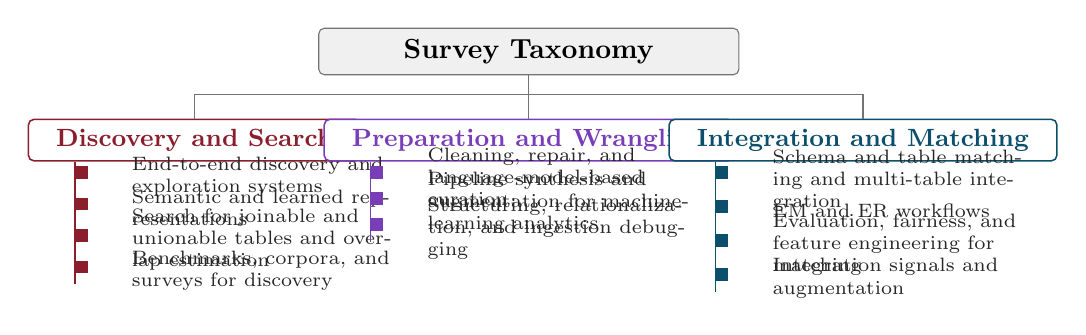
\begin{tikzpicture}[
  font=\scriptsize,
  >=Latex,
  conn/.style={draw=black!55, line width=0.45pt},
  title/.style={draw=black!55, rounded corners=2pt, fill=black!6,
                inner xsep=10pt, inner ysep=4pt, align=center,
                minimum width=0.44\textwidth},
  cat/.style={rounded corners=2pt, fill=white,
              inner xsep=10pt, inner ysep=3.5pt, align=center,
              minimum width=0.26\textwidth, line width=0.55pt},
  itemtext/.style={anchor=west, text=black!85, text width=0.27\textwidth}
]

\definecolor{discC}{HTML}{8B1E2D}
\definecolor{prepC}{HTML}{7A3DB8}
\definecolor{inteC}{HTML}{0B4F6C}

\def\bs{1.6mm}
\def\gapTop{5.5mm}
\def\barDrop{2.4mm}
\def\stem{2.2mm}
\def\ygap{3.3mm}
\def\discYgap{4.0mm}
\def\inteYgap{4.3mm}
\def\xoff{6.0mm}
\def\spineInset{6mm}

\node[title] (root) {\textbf{\normalsize Survey Taxonomy}};

\node[cat, draw=discC, text=discC, below=\gapTop of root, xshift=-0.35\textwidth] (disc)
  {\textbf{\small Discovery and Search}};
\node[cat, draw=prepC, text=prepC, below=\gapTop of root] (prep)
  {\textbf{\small Preparation and Wrangling}};
\node[cat, draw=inteC, text=inteC, below=\gapTop of root, xshift= 0.35\textwidth] (inte)
  {\textbf{\small Integration and Matching}};

\coordinate (barC) at ($(root.south)+(0,-\barDrop)$);
\coordinate (barL) at ($(disc.north |- barC)$);
\coordinate (barR) at ($(inte.north |- barC)$);

\draw[conn] (root.south) -- (barC);
\draw[conn] (barL) -- (barR);
\draw[conn] (barL) -- (disc.north);
\draw[conn] (barC) -- (prep.north);
\draw[conn] (barR) -- (inte.north);

\coordinate (discStem) at ($(disc.south west)+(\spineInset,0)$);
\coordinate (discB1)   at ($(discStem)+(0,-\stem)$);
\coordinate (discB2)   at ($(discB1)+(0,-\discYgap)$);
\coordinate (discB3)   at ($(discB2)+(0,-\discYgap)$);
\coordinate (discB4)   at ($(discB3)+(0,-\discYgap)$);

\draw[conn, draw=discC] (discStem) -- ($(discB4)+(0,-1.4mm)$);

\foreach \p/\txt in {
  discB1/{End-to-end discovery and exploration systems},
  discB2/{Semantic and learned representations},
  discB3/{Search for joinable and unionable tables and overlap estimation},
  discB4/{Benchmarks, corpora, and surveys for discovery}
}{
  \fill[discC] (\p) rectangle ++(\bs,\bs);
  \node[itemtext] at ($(\p)+(\xoff,0.3mm)$) {\txt};
}

\coordinate (prepStem) at ($(prep.south west)+(\spineInset,0)$);
\coordinate (prepB1)   at ($(prepStem)+(0,-\stem)$);
\coordinate (prepB2)   at ($(prepB1)+(0,-\ygap)$);
\coordinate (prepB3)   at ($(prepB2)+(0,-\ygap)$);

\draw[conn, draw=prepC] (prepStem) -- ($(prepB3)+(0,-1.4mm)$);

\foreach \p/\txt in {
  prepB1/{Cleaning, repair, and language-model-based curation},
  prepB2/{Pipeline synthesis and augmentation for machine-learning analytics},
  prepB3/{Structuring, relationalization, and ingestion debugging}
}{
  \fill[prepC] (\p) rectangle ++(\bs,\bs);
  \node[itemtext] at ($(\p)+(\xoff,0.3mm)$) {\txt};
}

\coordinate (inteStem) at ($(inte.south west)+(\spineInset,0)$);
\coordinate (inteB1)   at ($(inteStem)+(0,-\stem)$);
\coordinate (inteB2)   at ($(inteB1)+(0,-\inteYgap)$);
\coordinate (inteB3)   at ($(inteB2)+(0,-\inteYgap)$);
\coordinate (inteB4)   at ($(inteB3)+(0,-\inteYgap)$);

\draw[conn, draw=inteC] (inteStem) -- ($(inteB4)+(0,-1.4mm)$);

\fill[inteC] (inteB1) rectangle ++(\bs,\bs);
\node[itemtext] at ($(inteB1)+(\xoff,-0.2mm)$)
  {Schema and table matching and multi-table integration};

\foreach \p/\txt in {
  inteB2/{EM and ER workflows},
  inteB3/{Evaluation, fairness, and feature engineering for matching},
  inteB4/{Integration signals and augmentation}
}{
  \fill[inteC] (\p) rectangle ++(\bs,\bs);
  \node[itemtext] at ($(\p)+(\xoff,0.3mm)$) {\txt};
}

\end{tikzpicture}
\caption{Taxonomy of data lake research from discovery and search to analytics-ready outputs via preparation and integration.}
\label{fig:taxonomy}
\end{figure*}

\begin{table*}[t]
\caption{Phase-level summary of outputs, recurring tasks, and common concerns.}
\label{tab:phase-summary}
\centering
\tbl
\begin{tabularx}{\textwidth}{@{}p{29mm}p{34mm}Y p{45mm}@{}}
\toprule
\textbf{Phase} & \textbf{Primary output} & \textbf{Recurring tasks} & \textbf{Common concerns} \\
\midrule
Discovery and Search &
Ranked candidate tables, columns, views, or augmentations &
Keyword search, join search, union search, overlap estimation, view discovery, interactive exploration &
Weak metadata, large search space, ambiguity, index maintenance, and runtime cost \\
\addlinespace[0.25em]
Preparation and Wrangling &
Cleaned tables, structured views, transformed tables, or rerunnable workflows &
Repair, transformation recommendation, pipeline synthesis, feature augmentation, relationalization, ingestion debugging &
Unsafe edits, limited validation, repeatability, downstream utility, and evolving data \\
\addlinespace[0.25em]
Integration and Matching &
Column matches, entity matches, merge plans, reusable evidence, or merged outputs &
Schema matching, ER, blocking, merge-rule design, external augmentation, fairness auditing &
Supervision cost, partial overlap, fairness, privacy, policy constraints, and intent sensitivity \\
\bottomrule
\end{tabularx}
\end{table*}

\noindent Figure~\ref{fig:taxonomy} shows how the literature branches into subproblems, while the Table ~\ref{tab:phase-summary} shows what each branch actually produces for the next stage of the pipeline. Together they explain why the survey moves from finding candidate data, to stabilizing that data, to merging it into an analytics-ready result.

\subsection{Discovery and Search}
Discovery is the opening stage of the workflow: before any repair or integration can happen, the analyst needs a plausible set of candidate tables, columns, or views. Table~\ref{tab:discovery-methods} organizes this stage by showing how the literature moves from end-to-end search systems, to learned retrieval signals, to join/union relationship search, and finally to the shared resources that make discovery evaluation possible. The table is included to make the discovery taxonomy concrete and to show which paper families dominate this phase. Read it by category first, then by representative papers and the retrieval problems they emphasize.
\begin{table*}[!htbp]
\caption{Discovery \& Search papers mapped to taxonomy to show category structure and representative contributions.}
\label{tab:discovery-methods}
\tbl
\begin{tabularx}{\textwidth}{@{}p{24mm}p{28mm}p{18mm}Y@{}}
\toprule
\textbf{Category} & \textbf{Reference} & \textbf{Keywords} & \textbf{Contribution} \\
\midrule

End-to-end discovery and exploration systems &
CHORUS~\cite{10.14778/3659437.3659461} &
LMs, annotation &
Unifies multiple lake discovery/exploration tasks with a foundation-model pipeline and reports consistent gains over task-specific baselines. \\

~ &
BLEND~\cite{11112882} &
plans, ranking &
Defines a declarative discovery-plan abstraction that compiles to improved execution over heterogeneous signals for unified keyword, join, and union discovery with top-$k$ retrieval. \\

~ &
LakeCompass~\cite{10.14778/3685800.3685880} &
indexing, workflows &
End-to-end lake stack for maintenance, search, and analysis workflows, with scalable indexing and practical lake operations. \\

~ &
METAM~\cite{10184845} &
utility, ranking &
Ranks candidate datasets by expected downstream task utility through goal-aware profiling and ranking. \\

~ &
Selecting Sub-tables~\cite{10184535} &
sampling, previews &
Selects compact, informative sub-tables to accelerate inspection when full tables are too large or noisy. \\

~ &
Ver~\cite{10184768} &
views, interaction &
Question-driven view discovery that progressively prunes the space to surface useful derived tables. \\

\midrule

Semantic and learned representations &
CMDL~\cite{10.14778/3611479.3611533} &
cross-modal, embeddings &
Learns joint representations to retrieve across structured tables and unstructured text sources for cross-modal dataset discovery. \\

~ &
Starmie~\cite{10.14778/3587136.3587146} &
embeddings, contrastive &
Pretrains contextualized column representations that capture table context to improve semantic dataset discovery, especially unionable-table retrieval. \\

~ &
LIFTus~\cite{11113165} &
fusion, columns &
Learns multi-aspect column representations and adaptively fuses them to boost union search quality across heterogeneous lakes. \\

~ &
TabSketchFM~\cite{11113110} &
sketches, tokens &
Uses compact column sketches with a pretrained tabular model to scale discovery under token/compute constraints. \\

\midrule

Search for joinable and unionable tables and overlap estimation &
DeepJoin~\cite{10.14778/3603581.3603587} &
joinability, retrieval &
Pre-trained-language-model-based joinable-table discovery that embeds columns to rank candidate join partners, improving join discovery over lexical baselines. \\

~ &
SANTOS~\cite{10.1145/3588689} &
unionability, semantics &
Relationship-aware semantic union search using relational/context signals to find unionable tables with compatible meaning. \\

~ &
Nested/Joined Lake Search~\cite{10.14778/3681954.3682005} &
nested, joins &
Extends lake search to nested and join-derived candidates not well-modeled as flat standalone tables. \\

~ &
Armadillo~\cite{10.1145/3725365} &
overlap, graphs &
Learns table embeddings whose similarity approximates overlap ratio for fast scalable overlap estimation. \\

\midrule

Benchmarks, corpora, and surveys for discovery &
Rottnest~\cite{11113229} &
indexing, search &
Scalable lake indexing techniques to support efficient search over large, evolving lakes. \\

~ &
GitTables~\cite{10.1145/3588710} &
corpus, benchmark &
Large public corpus of relational tables mined at scale for reproducible training and evaluation. \\

~ &
LakeBench~\cite{10.14778/3659437.3659448} &
benchmark, labels &
Benchmark suite for joinable and unionable table discovery with ground-truth labeling at lake scale. \\

~ &
Data Discovery Survey~\cite{10.14778/3750601.3750694} &
survey, taxonomy &
Consolidates discovery operations across indexes and systems, and reviews evaluation practice while noting gaps in workloads and cost reporting. \\

~ &
Table Discovery Survey~\cite{10.1145/3555041.3589409} &
survey, methods &
Consolidated overview of table discovery methods and open directions at lake scale. \\

\bottomrule
\end{tabularx}
\end{table*}

Discovery research addresses the first bottleneck in data lakes: users may know the question they want to answer but still not know which tables are relevant, joinable, or worth inspecting. In practice, analysts usually begin with an information need such as ``find customer-address data'' or ``find tables that can enrich sales records,'' not with a precise table name. Discovery methods therefore combine three jobs: representing what a table contains, retrieving plausible candidates, and helping the user refine or trust the returned results.

The first category in Table~\ref{tab:discovery-methods} captures end-to-end systems such as LakeCompass, BLEND, CHORUS, METAM, Selecting Sub-tables, and Ver. These papers treat discovery as more than ranking. They maintain indexes, generate previews, support interaction, or optimize for downstream utility so that the analyst can decide whether a candidate should move deeper into the pipeline.

A second category replaces surface similarity with richer semantics. CMDL, Starmie, LIFTus, and TabSketchFM learn representations that remain useful when labels are sparse, abbreviated, or inconsistent. DeepJoin, SANTOS, Nested/Joined Lake Search, and Armadillo extend that shift to relationship search by ranking tables for joinability, unionability, or overlap rather than surface resemblance alone. In practice, these methods matter when lexical similarity is weak but the returned tables still need to support a later join, augmentation, or merge.

Discovery also depends on shared infrastructure. Rottnest, GitTables, and LakeBench support indexing, large-scale evaluation, and reproducible workloads, while the recent discovery surveys help stabilize terminology and task definitions. That support matters because strong ranking alone is not enough: discovery is only successful when the returned candidates reduce downstream preparation work instead of creating more of it.

\subsection{Preparation and Wrangling}
Once discovery has narrowed the lake, the survey moves to the middle stage: turning promising candidates into dependable inputs. Table~\ref{tab:prep-methods} connects papers that might otherwise look separate by showing that repair, workflow synthesis, relationalization, and ingestion debugging all answer the same question: how do we make selected data usable enough for later analysis and integration? The table is included to show that seemingly different papers are solving the same middle-stage usability problem. Read it by category first, then by representative papers and the kinds of usable outputs they try to produce.
\begin{table*}[!htbp]
\caption{Preparation \& Wrangling methods mapped to taxonomy to show category structure and representative contributions.}
\label{tab:prep-methods}
\tbl
\begin{tabularx}{\textwidth}{@{}p{24mm}p{28mm}p{18mm}Y@{}}
\toprule
\textbf{Category} & \textbf{Reference} & \textbf{Keywords} & \textbf{Contribution} \\
\midrule

Cleaning, repair, and language-model-based curation &
Automatic Data Repair~\cite{10.14778/3675034.3675051} &
repair, benchmark &
Benchmarks repair algorithms across datasets/error settings, proposes a repair-search strategy, and derives deployment guidelines. \\

~ &
DataRinse~\cite{10.14778/3611540.3611628} &
transforms, mining &
Recommends semantic data-prep transformations by mining data-preparation code repositories to learn reusable transformation patterns. \\

~ &
Foundation Models for Data Tasks~\cite{10.14778/3574245.3574258} &
LMs, prompting &
Casts classical cleaning/integration tasks as prompts and evaluates foundation models, noting strong generalization alongside privacy and domain-specific limitations. \\

~ &
Lingua Manga~\cite{10.14778/3611540.3611624} &
LLMs, templates &
Provides an LM-based curation system with modular templates and orchestration to run end-to-end curation workflows. \\

\midrule

Pipeline synthesis and augmentation for ML analytics &
CtxPipe~\cite{10.1145/3698831} &
pipelines, reinforcement learning (RL) &
Constructs preparation pipelines by conditioning operator selection on dataset/task context and using deep RL to search effective pipelines. \\

~ &
HAIPipe~\cite{10.1145/3588945} &
human-machine collaboration, reuse &
Combines human- and machine-generated pipelines via enumeration--sampling (with active learning) and uses RL to search improved machine-generated pipelines. \\

~ &
Featpilot~\cite{11113027} &
features, joins &
Automatically augments tabular datasets with useful additional features from joinable sources to improve downstream model performance. \\

~ &
Automatically Build Business-Intelligence Models (Auto-BI)~\cite{10.14778/3603581.3603596} &
BI, joins &
Predicts BI schema graphs (joins) via global search, evaluated on large collections of BI models. \\

\midrule

Structuring, relationalization, and ingestion debugging &
Evaporate~\cite{10.14778/3626292.3626294} &
views, synthesis &
Uses LMs plus lightweight synthesis and weak supervision to generate structured views over heterogeneous lake inputs. \\

~ &
Auto-Tables~\cite{10.1145/3665252.3665269} &
relationalization, schema &
Relationalizes semi-structured tables without examples by inferring structure/schemas and producing normalized relational output. \\

~ &
ReCG~\cite{10.14778/3681954.3682019} &
JavaScript Object Notation (JSON), clustering &
Discovers JSON schemas bottom-up by clustering records and generalizing clusters into schema fragments. \\

~ &
CM Explorer~\cite{10.14778/3611540.3611595} &
validation, debugging &
Disentangles correlated violated conditional unit tests using graph-based exploration to localize ingestion errors. \\

~ &
Fast and Scalable Data Transfer Across Data Systems~\cite{10.1145/3725294} &
transfer, tuning &
Decomposes data transfer into configurable stages and auto-tunes configurations for heterogeneous systems to improve throughput. \\

\bottomrule
\end{tabularx}
\end{table*}

Preparation and Wrangling changes the data itself. Where discovery returns a ranked list of candidates, preparation produces cleaned tables, derived features, structured views, or rerunnable workflows that can support repeated analysis. This stage matters because many errors that look small in isolation, such as inconsistent date formats or semi-structured headers, become serious blockers once matching or integration begins.

One major strand in Table~\ref{tab:prep-methods} emphasizes repair and transformation reuse. Automatic Data Repair focuses on safer repairs, DataRinse mines reusable transforms, foundation-model prompting broadens coverage across cleaning tasks, and Lingua Manga orchestrates end-to-end curation workflows. Across all four, the hard part is not generating candidate edits but checking whether those edits are correct, explainable, and repeatable.

Another strand treats preparation as workflow construction. CtxPipe, HAIPipe, Featpilot, and Auto-BI search for pipelines, join paths, or augmentations that improve recurring analytical tasks. Evaporate, Auto-Tables, ReCG, CM Explorer, and Fast and Scalable Data Transfer Across Data Systems instead focus on extracting structure from messy inputs, debugging ingestion failures, or tuning movement across systems. In these papers, preparation quality is measured less by local cleanliness than by whether the resulting tables are easier to analyze, join, or reuse.

Preparation therefore exposes a tension between quick automation and reusable process design. LM-based curation can shorten time to first result, but repeated use still requires provenance, validation, and rerunnable workflows. Pipeline-construction systems help when the same analytical pattern recurs across datasets, whereas relationalization systems matter when later matching depends on structure that is still implicit in the raw inputs.

\subsection{Integration and Matching}
Integration is the stage where cleaned candidates must become one coherent analytical output. Table~\ref{tab:integration-methods} groups this stage into schema/table integration, ER workflows, evaluation-oriented matching work, and reusable integration signals. The table is included to distinguish alignment evidence, workflow style, and merge concerns that otherwise get conflated in integration papers. Read it by category first, then by representative papers and the matching or merge issues each one foregrounds.
\begin{table*}[!htbp]
\caption{Integration \& Matching methods mapped to taxonomy to show category structure and representative contributions.}
\label{tab:integration-methods}
\tbl
\begin{tabularx}{\textwidth}{@{}p{24mm}p{28mm}p{18mm}Y@{}}
\toprule
\textbf{Category} & \textbf{Reference} & \textbf{Keywords} & \textbf{Contribution} \\
\midrule

Schema and table matching and multi-table integration &
DIALITE~\cite{10.1145/3555041.3589732} &
open-data, alignment &
End-to-end pipeline that discovers relevant open tables and integrates them by aligning schemas and values with knowledge-graph and LLM assistance. \\

~ &
ALITE~\cite{10.14778/3574245.3574274} &
integration, disjunction &
Adaptive-learning approach for integrating discovered lake tables under full-disjunction semantics at scale. \\

~ &
Magneto~\cite{10.14778/3742728.3742757} &
matching, hybrid LMs &
Hybrid schema-matching system: a smaller LM proposes candidate matches and a larger LM verifies or repairs ambiguous cases. \\

~ &
Pre-trained Language Model (PLM) Schema Matching~\cite{10184612} &
matching, embeddings &
Adapts PLMs to encode attribute and column semantics for schema matching across heterogeneous schemas. \\

\midrule

EM and ER workflows &
Flexible Entity Resolution (FlexER)~\cite{10.1145/3588722} &
ER, intents &
Models ER with multiple downstream intents as multi-label classification and uses a multiplex graph neural network (GNN) for intent-aware matching. \\

~ &
Progressive EM~\cite{10.1145/3709715} &
progressive, scheduling &
Characterizes the design space of progressive EM and benchmarks progressive strategies including neural-network- and PLM-based variants. \\

~ &
Unicorn~\cite{10.1145/3588938} &
multitask, matching &
Unified multi-task model supporting several DI matching tasks via shared encoders and task-specific heads. \\

~ &
WeakSup GT Inference~\cite{10.1145/3588712} &
weak-supervision, labels &
Infers latent ground truth from weak supervision sources by learning a label model that combines noisy signals for EM. \\

~ &
Battleship~\cite{10.1145/3626711} &
active-learning, low-resource &
Active-learning approach for low-resource EM that selects informative pairs via a Battleship-style strategy. \\

\midrule

Evaluation, fairness, and feature engineering for matching &
Fairness Lens~\cite{10.14778/3611479.3611525} &
fairness, bias &
Audits EM through fairness by constructing social datasets and analyzing disparate error rates under imbalance. \\

~ &
Filtering Benchmarks~\cite{10184692} &
blocking, benchmark &
Benchmarks combinations of filtering and scheduling strategies for progressive ER across datasets. \\

~ &
DescSim Rules~\cite{11112979} &
rules, features &
Introduces description-similarity rules to engineer informative, interpretable EM features from attribute descriptions. \\

~ &
Relation Enrichment~\cite{10.14778/3681954.3681987} &
enrichment, attributes &
Boosts ER quality by enriching related tuples with additional attributes from auxiliary sources. \\

\midrule

Integration signals and augmentation &
Causal Data Integration (CDI)~\cite{10.14778/3603581.3603602} &
causal, confounders &
Defines CDI by augmenting datasets with missing confounders from external sources and inferring a causal graph. \\

~ &
Entity Augmentation~\cite{10.14778/3611479.3611535} &
augmentation, querying &
Studies how to augment entities by selectively querying external sources with cost-aware querying strategies. \\

~ &
Sudowoodo~\cite{10184556} &
contrastive, representations &
Self-supervised contrastive approach that learns similarity-aware representations from unlabeled data and transfers to multiple DI tasks. \\

~ &
Similarity Inclusion Dependencies~\cite{10.1145/3588929} &
dependencies, profiling &
Discovers similarity inclusion dependencies, which act as approximate containment or foreign-key-like signals to reveal join and integration opportunities. \\

\bottomrule
\end{tabularx}
\end{table*}

What makes this stage difficult is not candidate retrieval but alignment under weak and partial evidence. In data lakes, metadata is often sparse, tables overlap only partially, and two analysts may want different definitions of what counts as the ``same'' entity or the ``same'' schema. Table~\ref{tab:integration-methods} therefore groups the literature by the kind of evidence each system uses before merging fragments.

DIALITE and ALITE keep merge semantics in view after discovery, while Magneto and the PLM schema-matching method strengthen alignment with LM or embedding signals. In all four cases, a column match is only an intermediate result: the system still has to decide how partial tuples, open-world values, and schema differences are carried into the merged output.

FlexER, Progressive EM, Unicorn, WeakSup GT Inference, and Battleship treat matching as workflow design under varying intents, budgets, and supervision levels. The surrounding papers in this section add fairness audits, blocking benchmarks, feature rules, enrichment methods, external augmentation, self-supervised representations, causal augmentation, and similarity constraints. The result is a body of work that studies not only how to classify a pair, but also which signals should be collected and trusted before a merge is accepted.

Correctness is also highly task dependent at this stage. A merged result can be technically well aligned but still analytically wrong if it collapses partial evidence, applies the wrong entity granularity, or hides ambiguity that a user would want to inspect. Recent matching work therefore spends more attention on intent, fairness, supervision cost, and reusable evidence, not only on final accuracy.

\section{Comparison and Discussion}
By this point, the earlier tables have introduced the major method families phase by phase. Table~\ref{tab:comparison} brings them back together and asks the higher-level survey question: under what scenarios does each family help most, and where do its strengths stop being enough?
\begin{table*}[t]
\caption{Cross-phase comparison of representative method families.}
\label{tab:comparison}
\centering
\tbl
\begin{tabularx}{\textwidth}{@{}p{28mm}p{34mm}Y Y Y@{}}
\toprule
\textbf{Family} & \textbf{Representative works} & \textbf{Works well when} & \textbf{Main strengths} & \textbf{Main limitations} \\
\midrule
End-to-end discovery systems &
LakeCompass~\cite{10.14778/3685800.3685880}, BLEND~\cite{11112882}, CHORUS~\cite{10.14778/3659437.3659461} &
Users need broad search over large lakes &
Unified search and exploration stack &
Maintenance cost and intent drift \\
\addlinespace[0.25em]
Learned discovery and relationship search &
Starmie~\cite{10.14778/3587136.3587146}, DeepJoin~\cite{10.14778/3603581.3603587}, SANTOS~\cite{10.1145/3588689} &
Semantic overlap matters more than exact names &
Robust to weak metadata &
Training cost and lower interpretability \\
\addlinespace[0.25em]
Cleaning and workflow automation &
Automatic Data Repair~\cite{10.14778/3675034.3675051}, CtxPipe~\cite{10.1145/3698831}, Lingua Manga~\cite{10.14778/3611540.3611624} &
Preparation tasks repeat across datasets &
Reusable workflows and less manual work &
Hard validation and unsafe edits \\
\addlinespace[0.25em]
Structuring and relationalization &
Evaporate~\cite{10.14778/3626292.3626294}, Auto-Tables~\cite{10.1145/3665252.3665269}, ReCG~\cite{10.14778/3681954.3682019} &
Inputs are semi-structured or irregular &
Makes messy data queryable &
Brittle multi-step transforms \\
\addlinespace[0.25em]
Integration and ER workflows &
DIALITE~\cite{10.1145/3555041.3589732}, Magneto~\cite{10.14778/3742728.3742757}, FlexER~\cite{10.1145/3588722}, Unicorn~\cite{10.1145/3588938} &
Sources overlap under limited labels or policy constraints &
Richer outputs and intent awareness &
Merge semantics, fairness, and privacy \\
\bottomrule
\end{tabularx}
\end{table*}

Table~\ref{tab:comparison} shows that the major method families solve different bottlenecks and should be compared by scenario rather than by one universal metric. Discovery families help when the lake is large and weakly documented, preparation families matter when cleaning logic or workflow structure must be reused, and integration families matter when partial overlap, ambiguous matches, or policy constraints dominate.

This comparison also clarifies why older design choices remain relevant. Metadata-driven discovery is still attractive when lakes are stable and descriptive, rule-based repair remains useful when strong domain constraints are available, and explicit merge semantics remain valuable when partial facts must be preserved. Learned methods become more attractive when labels are sparse, schemas vary, or semantics drift across sources, but they usually demand more validation, more compute, and more user trust.

Within discovery, the main contrast is between operational breadth and semantic depth. Systems centered on indexes, plans, and previews are often easier to monitor and maintain, and they work well when table names, keys, or metadata remain reasonably informative over time. Learned retrieval becomes more valuable when those signals are weak or inconsistent, because column content and context carry more meaning than names alone. The trade-off is that explanations become harder. A user may receive a strong candidate without understanding which structural or semantic cues made it appear reliable, which can slow trust and downstream adoption.

Preparation methods divide more sharply by intended use. Repair and transformation systems are most effective when analysts repeatedly confront noisy values, format inconsistencies, or missing fields. Pipeline-synthesis systems are better suited to repeated ML or BI tasks where reusable operator sequences matter as much as the final table. Structuring and relationalization systems solve a different problem again: they create the tabular form that later discovery and matching methods assume already exists. In practice, one family is not ``better'' than another unless the analyst's bottleneck is clear, because each family removes a different source of difficulty.

Integration methods also differ in where their difficulty lies. Some problems are dominated by schema heterogeneity and benefit from stronger column representations or staged matching. Others are dominated by limited labels, so weak supervision, active learning, or reusable similarity signals become more useful than a slightly stronger final classifier. In settings with partial overlap, open data, or enterprise policy constraints, explicit merge semantics may matter more than raw matching accuracy. A system that exposes how partial facts are preserved can be more valuable than one that reports a higher score but hides important modeling assumptions.

Across all three phases, the key question is whether a method leaves the next stage easier rather than harder.

\section{Open Challenges and Future Directions}
\paragraph{End-to-End Evaluation.}
Most papers still report metrics for a single phase. A major need is benchmark design that records stage-level metrics together with at least one end-to-end analytical outcome; without that broader view, phase-specific scores can make methods look more comparable than they really are.

\paragraph{Intent, Interaction, and Safe Automation.}
Analytical intent is often ambiguous in data lakes, so future systems should support interactive refinement and make uncertainty visible instead of hiding it. This matters even more as language-model-based discovery, preparation, and integration become common. The open problem is not only how to automate more, but how to automate safely through validation hooks, rollback mechanisms, constraint checks, and confidence-aware execution. Analysts should be able to inspect competing joins, repairs, and match definitions before those choices become part of a final dataset.

\paragraph{Scale, Maintenance, and Governance.}
At realistic lake scale, infrastructure costs matter as much as model quality. Discovery systems must maintain indexes and embeddings, preparation systems may execute many candidate workflows, and integration systems often spend most of their time in blocking, filtering, or label acquisition. Future work should therefore report runtime-quality trade-offs explicitly and treat governance, fairness, and privacy rules as planning constraints rather than as after-the-fact filters. Incremental maintenance is especially important when lakes evolve continuously instead of by occasional rebuilds.

\paragraph{Evolving Lakes and Shared Resources.}
Many systems still assume that the analytical challenge begins only after data has already been made tabular, but real lakes evolve in format, nesting depth, and storage location over time. Future work should connect discovery, preparation, and integration more directly for semi-structured and changing data. It also needs shared test collections that cover the full pipeline, maintenance cost, and boundary failures under evolving-lake conditions.

\section{Conclusion}
Recent data-lake research now supports a clear three-phase view: discovery narrows the search space, preparation stabilizes candidate data, and integration aligns and merges the final sources. The main lesson is practical rather than taxonomic: systems should be judged by how reliably they turn retrieved candidates into usable analytical datasets, especially when automation, intent, and governance interact across phase boundaries.

\bibliographystyle{ACM-Reference-Format}
\bibliography{ref}

\end{document}
